
\section{VALIDATION}
\label{sec:validation}
\subsection{Experimental Setup}
% hardware setup
To validate the performance of the proposed framework for assessing lifting risk in a real-time application, an experimental analysis is performed in a laboratory environment. A healthy volunteer is asked to perform three different lifting tasks corresponding to varied risk levels. In this setup, the participant’s kinematics state is collected using \emph{iFeel}, which is composed of a set of \emph{iFeel-Nodes} (including sensors and actuators) and a central processing unit \emph{iFeel-Station} (a micro-controlled board). The system operates for whole-body motion tracking via \emph{iFeel-Nodes} that are mounted in pre-defined locations of the \emph{iFeel-Suit}. Each \emph{iFeel-Node} contains a 9-DoF IMU that provides absolute orientation and sensor-based velocity fusion data at a rate of 100 Hz. Once detecting any possible risks, a signal is sent to the haptic actuator of the \emph{ifeel node} mounted on the human waist. The ground reaction forces and torques are retrieved using \emph{iFeel-Shoes} equipped with F/T sensors integrated in the front and rear parts. The collected human data are streamed and resampled via YARP middleware \cite{Metta2006} at a rate of 100Hz. Moreover, as mentioned in section \ref{sec:human_modeling_estimation}, human is modeled as a floating-base multi-rigid-body system considering 13 joints (e.g. T9T8, Right shoulder, etc.). The programs run on a 64-bit i7 2.6GHz laptop which is equipped with 32 GB RAM, Intel(R) UHD Graphics and Ubuntu 20.04 LTS. 

% task design
The parameters of performed lifting tasks are listed in Table \ref{tab:task_data}. Specifically, asymmetry angle A equals zero (AM = 1.0), coupling quality is \emph{Fair} (CM = 0.95), and lifting frequency is controlled as 7 lifts/min (FM = 0.7). The payload is evenly distributed inside a square box and the weight value is sent to the framework as an external parameter from the user. 
% Please add the following required packages to your document preamble:
% \usepackage{multirow}
\begin{table}[]
\centering
\caption{Experimental lifting task variables of RNLE.}
\resizebox{\columnwidth}{!}{%
\begin{tabular}{|c|cclccccc|cc|}
\hline
\multirow{3}{*}{\textbf{\begin{tabular}[c]{@{}c@{}}Task\\ type\end{tabular}}} &
  \multicolumn{8}{c|}{\textbf{RNLE variables}} &
  \multicolumn{2}{c|}{\textbf{RNLE results}} \\ \cline{2-11} 
 &
  \begin{tabular}[c]{@{}c@{}}H\_origin\\ (cm)\end{tabular} &
  \multicolumn{2}{c}{\begin{tabular}[c]{@{}c@{}}H\_end\\ (cm)\end{tabular}} &
  \begin{tabular}[c]{@{}c@{}}V\_origin\\ (cm)\end{tabular} &
  \begin{tabular}[c]{@{}c@{}}V\_end\\ (cm)\end{tabular} &
  \begin{tabular}[c]{@{}c@{}}D\_origin\\ (cm)\end{tabular} &
  \multicolumn{1}{c|}{\begin{tabular}[c]{@{}c@{}}D\_end\\ (cm)\end{tabular}} &
  \multirow{2}{*}{\begin{tabular}[c]{@{}c@{}}L\\ (kg)\end{tabular}} &
  \multicolumn{1}{c|}{\begin{tabular}[c]{@{}c@{}}RWL\_origin\\ (kg)\end{tabular}} &
  \multirow{2}{*}{LI} \\ \cline{2-8} \cline{10-10}
 &
  \multicolumn{1}{l}{HM\_origin} &
  \multicolumn{2}{l}{HM\_end} &
  \multicolumn{1}{l}{VM\_origin} &
  \multicolumn{1}{l}{VM\_end} &
  \multicolumn{1}{l}{DM\_origin} &
  \multicolumn{1}{l|}{DM\_end} &
   &
  \multicolumn{1}{c|}{\begin{tabular}[c]{@{}c@{}}RWL\_end\\ (kg)\end{tabular}} &
   \\ \hline
\multirow{2}{*}{Task 1} &
  47 &
  \multicolumn{2}{c}{63} &
  8 &
  68 &
  60 &
  \multicolumn{1}{c|}{60} &
  \multirow{2}{*}{3} &
  \multicolumn{1}{c|}{5.84} &
  0.51 \\
 &
  0.53 &
  \multicolumn{2}{c}{0.40} &
  0.80 &
  0.98 &
  0.90 &
  \multicolumn{1}{c|}{0.90} &
   &
  \multicolumn{1}{c|}{5.40} &
  0.56 \\ \hline
\multirow{2}{*}{Task 2} &
  47 &
  \multicolumn{2}{c}{63} &
  8 &
  80 &
  72 &
  \multicolumn{1}{c|}{72} &
  \multirow{2}{*}{7} &
  \multicolumn{1}{c|}{5.71} &
  1.23 \\
 &
  0.53 &
  \multicolumn{2}{c}{0.40} &
  0.80 &
  0.99 &
  0.88 &
  \multicolumn{1}{c|}{0.88} &
   &
  \multicolumn{1}{c|}{5.33} &
  1.31 \\ \hline
\multicolumn{1}{|l|}{\multirow{2}{*}{Task 3}} &
  47 &
  \multicolumn{2}{c}{63} &
  8 &
  92 &
  83 &
  \multicolumn{1}{c|}{83} &
  \multirow{2}{*}{10} &
  \multicolumn{1}{c|}{5.64} &
  1.77 \\
\multicolumn{1}{|l|}{} &
  0.53 &
  \multicolumn{2}{c}{0.40} &
  0.80 &
  0.95 &
  0.87 &
  \multicolumn{1}{c|}{0.87} &
   &
  \multicolumn{1}{c|}{5.06} &
  1.98 \\ \hline
\end{tabular}
\label{tab:task_data}
}
\end{table}
% task execution
During the experiment, the participant is asked to repeat each task three times as steady and natural as possible, such that no jerks appear during lifting. The participant should avoid twisting the upper trunk so that the assumption of zero asymmetry angle is fulfilled. Furthermore, the participant is required to hold the box with both hands while his feet are maintained in a fixed position. The lifting activity is executed slowly, hence every single execution can be regarded as independent from the others. 

\subsection{Results and Discussion}
In this section, we first performed a variety of quantitative evaluations of the adapted GMoE model using an additionally collected unseen dataset, which is in a total of 15248 frames. Then we conducted a qualitative analysis based on the results of previously designed online experiments. 
\subsubsection{Quantitative Evaluation of Action Recognition}
\label{sec: analysis action recognition}
% address the concern of overfitting when using a small dataset via quantitative evaluation of action recognition and motion prediction
% action recognition metrics
% 1) Accuracy: true positive for each action label
% 2) Fastness: how fast can an action change be detected (do we need this metric??)
In order to assess the action classification performance, a confusion matrix associated with three human lifting actions is presented in Figure \ref{fig:confusion_matrix}.
Based on this confusion matrix, metrics such as \emph{Accuracy}, \emph{Precision}, \emph{Recall} and \emph{F1 score} can be further retrieved. \emph{Accuracy} is the number of correct predictions of all \emph{N} categories divided by the total number of predictions, as shown in Equation \ref{accuracy}, where \emph{total} means the number of all tested samples.
\begin{equation} \label{accuracy}
\begin{split}
Accuracy = \frac{\sum_{i=1}^{N}TP_i}{total}
\end{split}
\end{equation}

\emph{Precision} refers to the proportion of correctly predicted positive instances out of all instances predicted as positive, while \emph{Recall} measures the proportion of correctly predicted positive instances out of all actual positive instances, as shown in Equation \ref{precision} and \ref{recall}, where \emph{i} means each class.
\begin{subequations}
\begin{align} \label{precision}
& Precision = \frac{TP_i}{TP_i + FP_i} ~,\\
\label{recall}
& Recall = \frac{TP_i}{TP_i + FN_i} ~.
\end{align}
\end{subequations}

\emph{F1 score} can be interpreted as a harmonic mean of the \emph{Precision} and \emph{Recall} as shown in Equation \ref{F1_score}.
\begin{equation} \label{F1_score}
\begin{split}
F1 = \frac{2 * Presicion * Recall}{Precision + Recall}
\end{split}
\end{equation}

\begin{figure}[t]
   \centering
   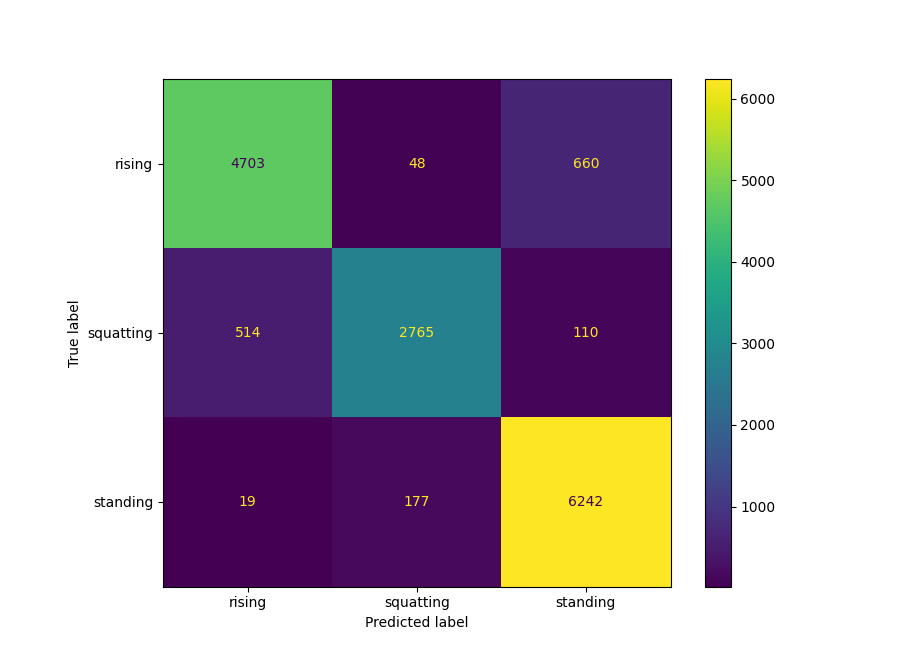
\includegraphics[scale=0.4,trim={1cm 0 5.3cm 2cm},clip]{figures/cm01.png}
   \caption{Confusion matrix for the action classification.}
   \label{fig:confusion_matrix}
\end{figure}

Table \ref{tab:metrics} summarizes the experimental results of these metrics for each single category classification.
% Please add the following required packages to your document preamble:
% \usepackage{multirow}\centering
\begin{table}[b]
\centering
\caption{Performance metrics for assessing GMoE model recognizing multi-class human lifting actions.}
\resizebox{\columnwidth}{!}{%
\begin{tabular}{|c|c|c|c|c|}
\hline
\multicolumn{1}{|l|}{} & \textbf{Accuracy} & \textbf{Precision} & \textbf{Recall} & \textbf{F1 score} \\ \hline
\textit{standing}  & \multirow{3}{*}{/} & 0.890 & 0.969 & 0.928 \\ \cline{1-1} \cline{3-5} 
\textit{rising}    &                    & 0.898 & 0.869 & 0.883 \\ \cline{1-1} \cline{3-5} 
\textit{squatting} &                    & 0.925 & 0.816 & 0.867 \\ \hline
\textit{average}   & 0.899              & 0.904 & 0.885 & 0.893 \\ \hline
\end{tabular}
\label{tab:metrics}
}
\end{table}
As we can see, \emph{squatting} has the highest accuracy of 0.925, which indicates that the model has a low rate of falsely labeling instances as this action. On the contrary, \emph{standing} has a relatively low accuracy. This is mainly because the transition period between \emph{rising} and \emph{standing} can be quite ambiguous (also partly due to the fact that the annotated border depends on human judgment), such that it can be hard for the model to distinguish these two phases exactly. Furthermore, both \emph{squatting} and \emph{rising} have relatively lower \emph{Recall} values than \emph{standing}. As explained before, the ambiguity between \emph{rising} and \emph{standing} leads to some false labeling of \emph{standing} when they are actually \emph{rising}. Also, the similarity between the motion patterns of \emph{squatting} and \emph{rising} (they are basically reversed) results in the confusion of them.

\subsubsection{Quantitative Evaluation of Motion Prediction}
\label{sec: analysis motion prediction}
% accuracy of motion prediction (multiple joints)
In the following, we report the performance of GMoE regarding the task of motion prediction. Two key joints (i.e., left knee and right elbow) that can reflect respectively the human upper-/lowerbody motion patterns during a lifting task are chosen. The rotational angles around the y-axis of these two joints during a period of about 5500 frames are demonstrated in Figure \ref{fig:motion_predictions}. The ground truths are depicted in black curves, while the predicted angles at the future time steps 0, 19 and 49 are shown respectively in blue, orange and yellow.
\begin{figure}[t]
   \centering
   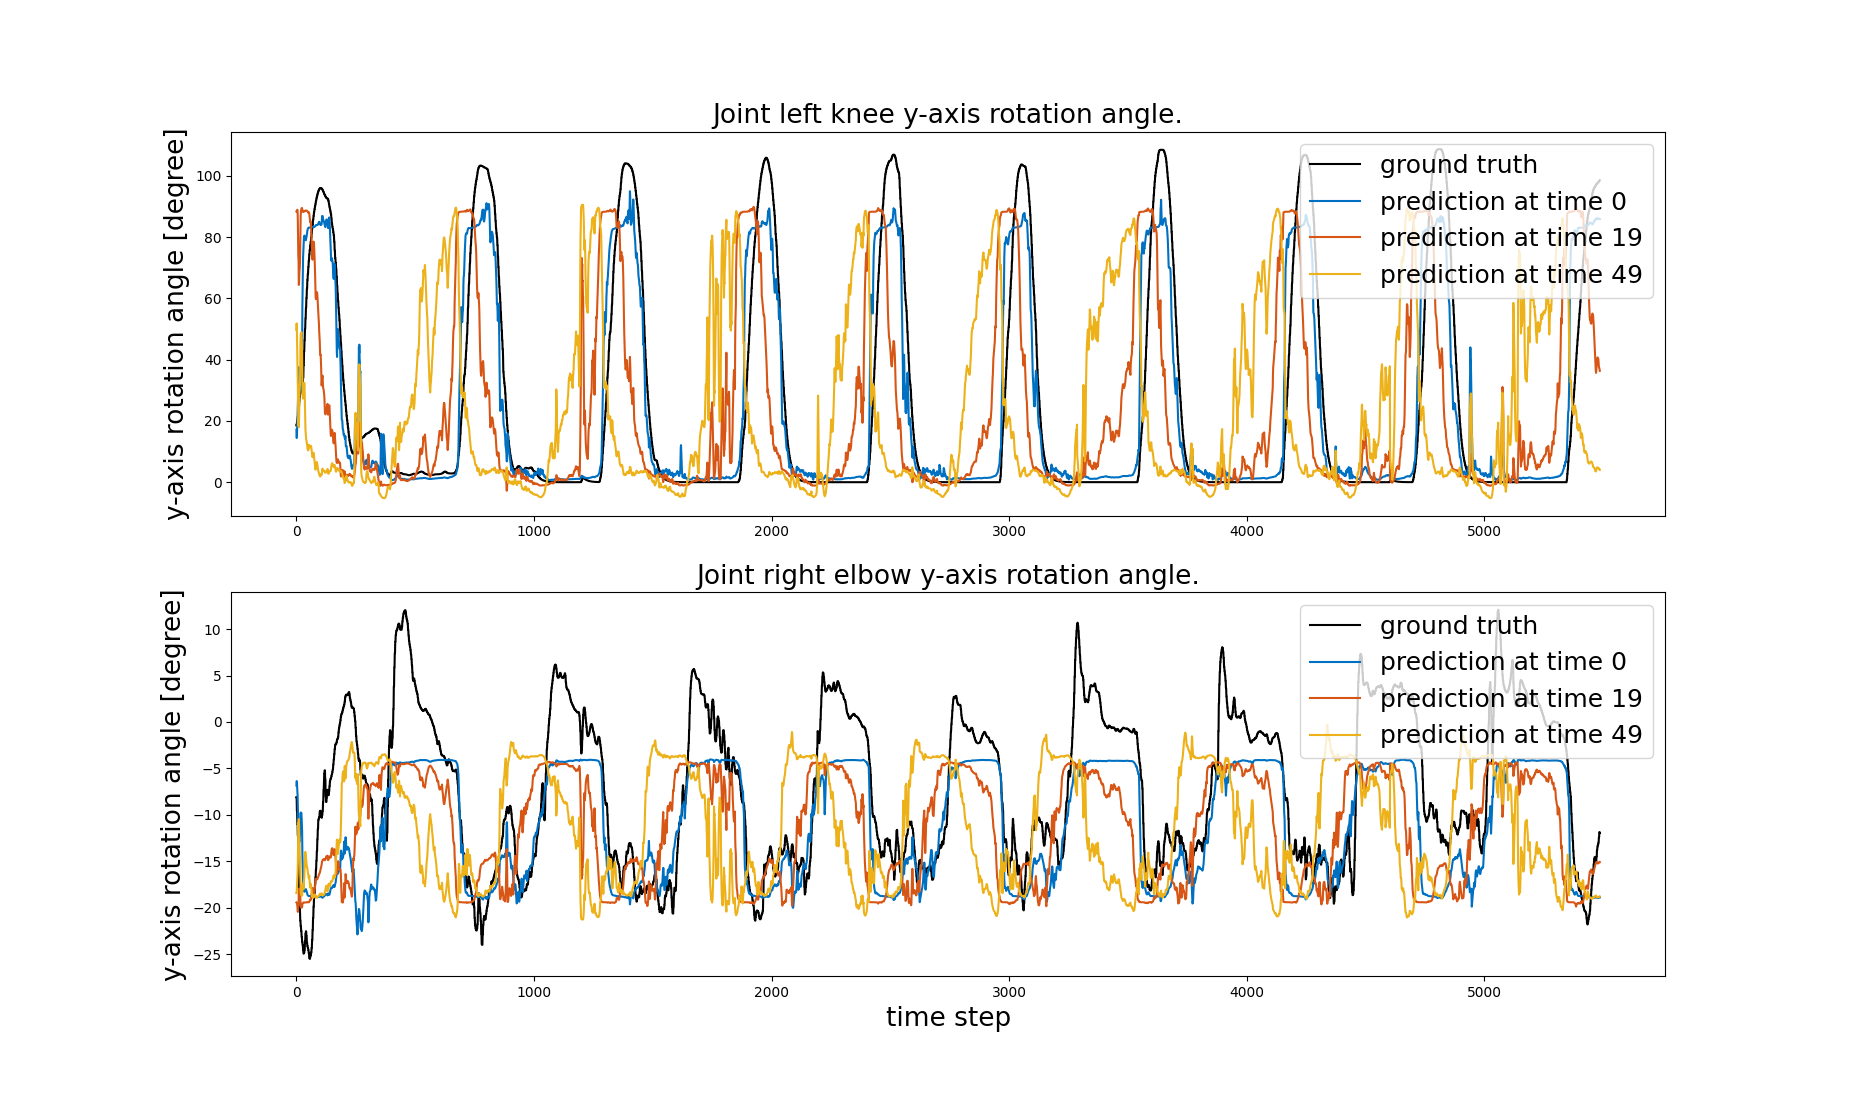
\includegraphics[width=1.1\columnwidth]{figures/motion_predictions02.png}
   \caption{Multi-time-step predictions of the y-axis rotation angle of the joint left knee and right elbow.}
   \label{fig:motion_predictions}
\end{figure}

It can be observed from both rows in Figure \ref{fig:motion_predictions} that the predicted y-axis rotational angle at future time step 0 (blue curves) basically captures the motion pattern of the ground truths (black curves), despite the amplitude gaps at peaks. The amplitude differences at peak positions can be more easily observed for the right elbow joint. The predicted rotational angles at future time steps 19 and 49 exhibit a leading phase compared with the ground truth, where the phase differences should match the corresponding prediction time steps. It should be noted that the predictions at future time step 49 suffer more from uncertainties, which is reflected by the frequently appearing sharp fluctuations. This may be due to the fact that the model only has very limited historical information, yet to make a further prediction in the future, it is apparently insufficient to solely rely on this short period of history. Another interesting fact is that the model seems to perform worse in predicting the motions of the right elbow joint. A possible reason could be that the movements of the right elbow are also affected by the pose of the pelvis, while the knees have a more independent thus also more predictable motion pattern.


\subsubsection{Qualitative Evaluation}
\label{sec: qualitative evaluation}
% TO DO: highlight haptic alert and mention the benefits of doing so 
To further evaluate the effectiveness of the proposed framework, we analyze qualitatively the results of \emph{Task 2} (shown in Table \ref{tab:task_data}) as an example. A complete process of \emph{rising} is demonstrated in Figure \ref{fig:resutls}. As shown in the first row, the motions of both real human subject and simulated models are captured. The grey model reconstructs the human motion at current time \emph{t} from sensor measurements, while the red model represents the predicted human motion at future time \emph{t+0.6s} (in the experiment we output the maximum future 20 data frames, recalling the period between each data frame is 30ms, thus the prediction time is 0.6s). The correspondingly recognized actions at each moment are presented in the second row. The black, blue and red solid curves denote the probability of action \emph{rising}, \emph{squatting} and \emph{standing}, respectively. In the third row, we demonstrate the predictions of rotation degrees of left knee joint around \emph{y}-axis for future 1.5s (maximum 50 future data frames), associated with the round dot curves. In the meanwhile, the blue curve stands for the ground truth of left knee joint rotation values. Figures in the last row demonstrate the lifting index during the \emph{rising} action. The red curve and grey dot curve represent the risk value at the current time and future 0.9s (namely 30 data frames), respectively.
% TO DO: point out where the haptic alert is activated
\begin{figure*}[h]
    \centering
    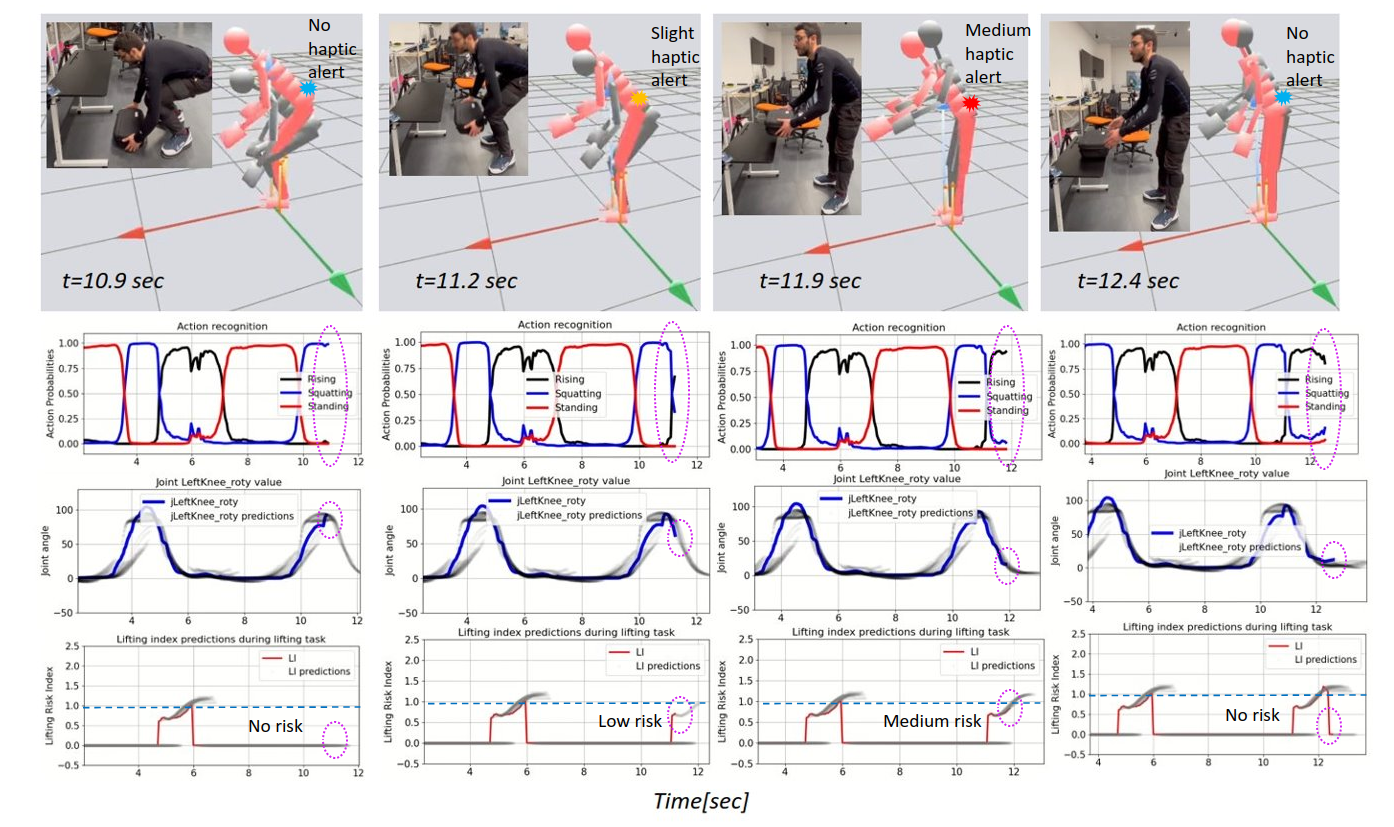
\includegraphics[width=1.0\textwidth]{figures/modified_qualitative_plot.png}
    \caption{Experimental results of online action recognition and risk prediction. The first row shows pictures of the sensorized subject during the task execution and virtual model visualization with estimated (gray) and predicted (red) configuration. In the second row, it is shown the action prediction probability. In the third row, ground truth and prediction of the left knee joint rotation angle are depicted. The bottom row shoes lifting index for the period till prediction time horizon.}
    \label{fig:resutls}
\end{figure*}

As shown in the picture at the top left in Figure \ref{fig:resutls}, the human is almost finishing the action \emph{squatting} at t=10.9s, and as the red model indicates, at the future time t=11.5s, the human model would probably be rising up a little bit. The recognized action at t=10.9s is still \emph{squatting}, therefore no lifting risk is detected and the haptic actuator remains silent. As for the rotation angle of the left knee joint, it also reaches a peak value of about 100 degrees and it's going to decrease soon. When time t becomes 11.2s, it can be observed that the gray model is reaching the pose as predicted at t=10.9s. In the meanwhile, the action transition already started, thus we can see that the lifting risk grows from zero to 0.7 (hence a slight haptic alert appears), and as the predictions show, the risk value at t=11.8s should be equal to 1.0. Then at t=11.9s, the human is reaching the table and intends to put the payload on it. At this moment, the action is still recognized as \emph{rising} with maximum probability. Moreover, the currently estimated lifting index is around 0.9 (corresponding to a medium haptic warning), which almost equals the value predicted at t=11.2s. At the final time t=12.4, apparently the \emph{rising} action is completed, and the human subject is getting back to \emph{standing} pose. Therefore the probability of \emph{rising} starts to decrease. Correspondingly, the lifting index returns back to zero again.

%For the other two tasks, all the pipelines showed similar performance. Based on the results of conducted online tests, the proposed framework can satisfy the basic requirements for estimating and predicting lifting-related hazards in a real-time application, hence the human subject is also aware of potential risks via haptic feedback from the wearables. 

\subsubsection{Failure Cases}
% failure case or say limitations: 
% - totally unseen motions
% - not applicable to collaborative lifting
% - accumulated noise and perturbations
% - retrieve NIOSH variables precisely
We present some failure cases here to reveal the limitations of the current system. As explained in Section \ref{subsec:make_data}, the GMoE network is trained on a 15-mins data set that consists of basic lifting tasks. Hence, a very typical unsuccessful scenario is when completely unseen motion patterns appear in the online application, e.g., trunk twisting and overhead lifting. In such cases, precise action detection can become an issue, let alone predict risks. Additionally, the GMoE model can be further generalized when trained on a dataset with multiple individuals (e.g., age, gender, body shape and etc). Another challenge lies in the restrictions of the NIOSH equation.  For example, the system is not applicable to collaborative lifting tasks where multiple workers are present. Moreover, the noise and perturbations accumulated over time in online applications also have a great effect on the accuracy of the GMoE model. We hypothesize that the retrievement of unprecise NIOSH variables is also a notable limitation. This is the main reason for improving the swiftness of action detection and the accuracy of motion predictions. 


\subsection{Discussion}
% TO DO: advantage of risk assessment and prediction compared to SOTA
% TO DO: benefits of haptic alerting during the task
In comparison to risk assessment approaches proposed in literature \cite{Shafti2019, Fortini2020ROMAN, fortini2020framework}, the main advantage of the proposed framework lies in its ability to early assessment and prevention of biomechanical risks faced by workers during realistic lifting tasks, by utilizing a learning-based approach and wearable sensing system. Despite training on a relatively small data set, we have shown that our model is able to generalize well to unseen data (though restricted to the same motion patterns that appeared in the training dataset), as analyzed in \ref{sec: analysis action recognition} and \ref{sec: analysis motion prediction}. We also demonstrate robust qualitative performance during the live demo presented in \ref{sec: qualitative evaluation}. It is worth mentioning that although humans can feel muscular fatigue in the long term, the causal action is often neglected due to the lack of real-time quantitative ergonomic feedback. Therefore the anticipated haptic alerts is very potentially to improve the risk awareness of workers while performing heavy lifting tasks.








